\section{Approximate Abstraction on Example Domains}

Here we discuss the results shown in states blah blah \dnote{Description of this section}.


\begin{itemize}
\item For $\epsilon > 0$, there are extremely useful abstractions to be made. Want to emphasize that with approximate knowledge of X, can still abstract effectively (point out Minefield + NChain both retain a very good policy from abstract MDP). This hits the learnable point.
\item Explain goal based/Taxi (regenerate plot for different scale of epsilon)
\item Possibly talk about stochasticity (low priority)
\item Explain Random behavior, smooth interpolation, mention randomness, etc.
\item Describe plots a bit (what is the y-axis?)
\end{itemize}

% Figure: Epsilon vs. #States for all three sample domains.
\begin{figure}
\centering

\subfigure[NChain]{
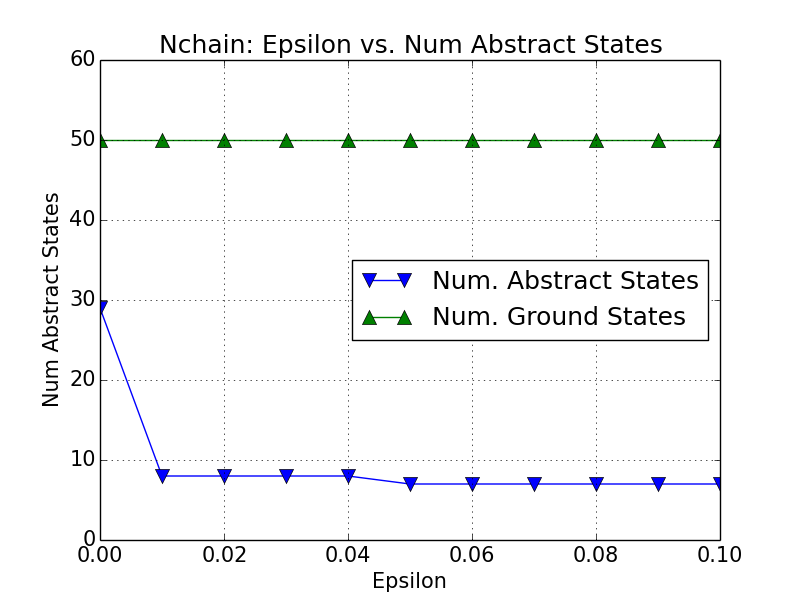
\includegraphics[width=0.46\columnwidth]{figures/nchain_epsilon_vs_num_abstract_states.png}
}
\subfigure[NChain]{
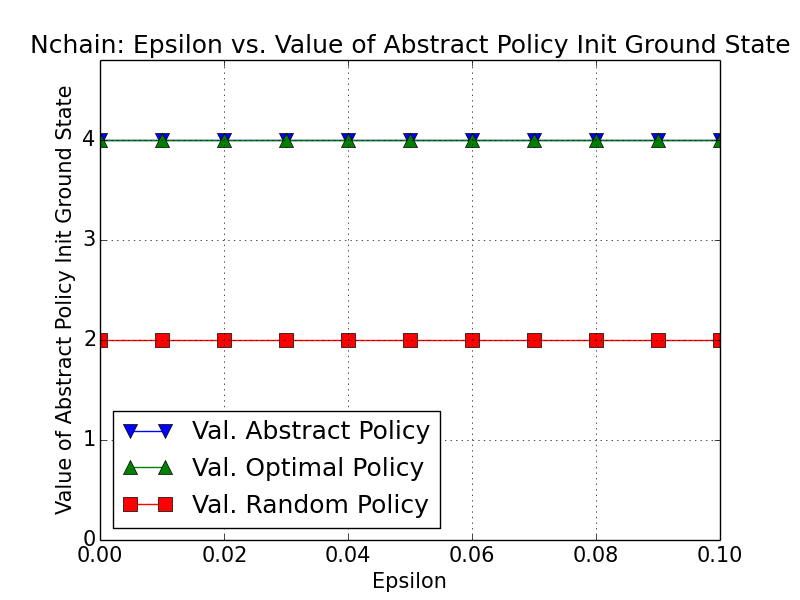
\includegraphics[width=0.46\columnwidth]{figures/nchain_epsilon_vs_value_of_abstract_policy_init_ground_state.png}
}

\subfigure[Taxi]{
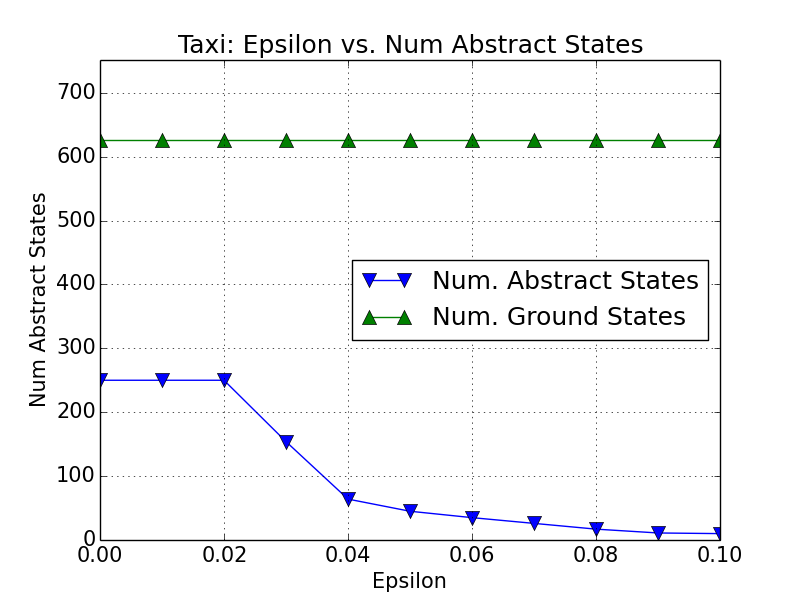
\includegraphics[width=0.46\columnwidth]{figures/taxi_epsilon_vs_num_abstract_states.png}
}
\subfigure[Taxi]{
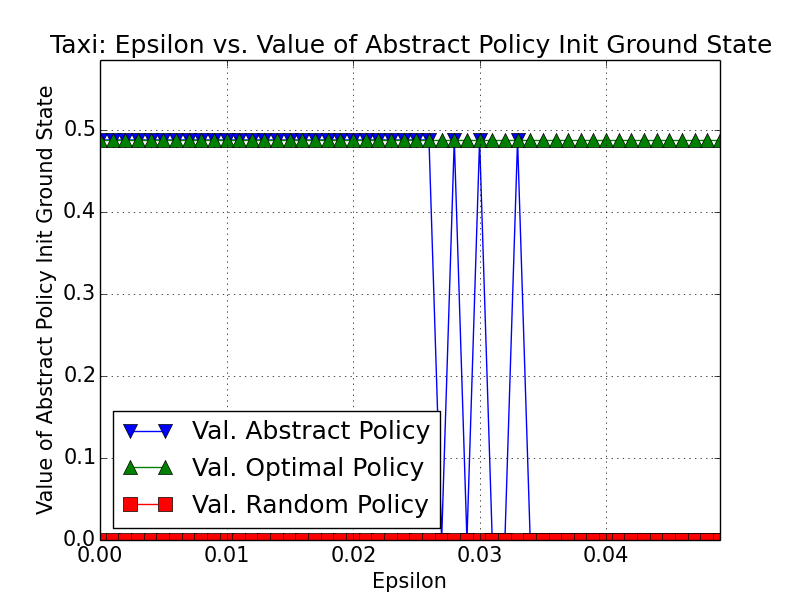
\includegraphics[width=0.46\columnwidth]{figures/taxi_epsilon_vs_value_of_abstract_policy_init_ground_state.png}
}

\subfigure[Minefield]{
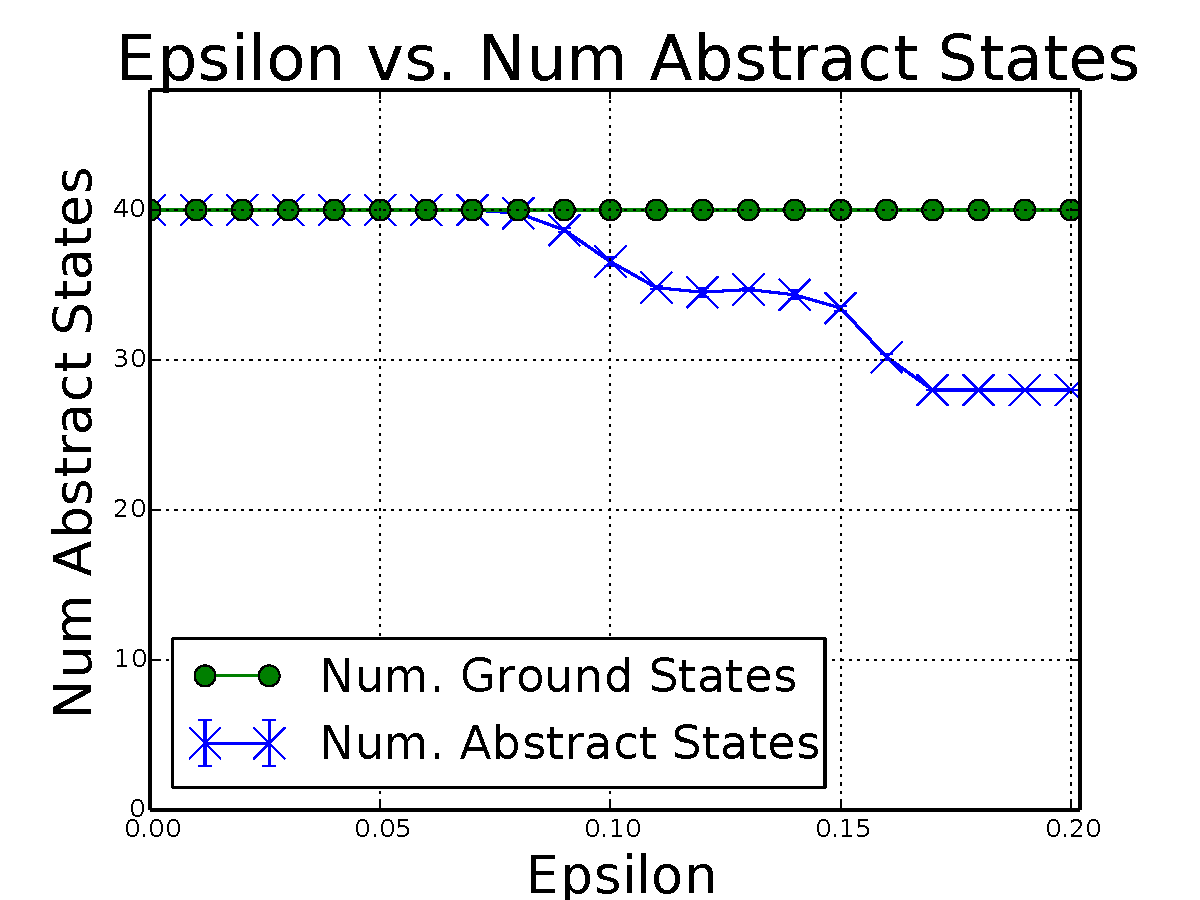
\includegraphics[width=0.46\columnwidth]{figures/minefield_epsilon_vs_num_abstract_states.pdf}
}
\subfigure[Minefield]{
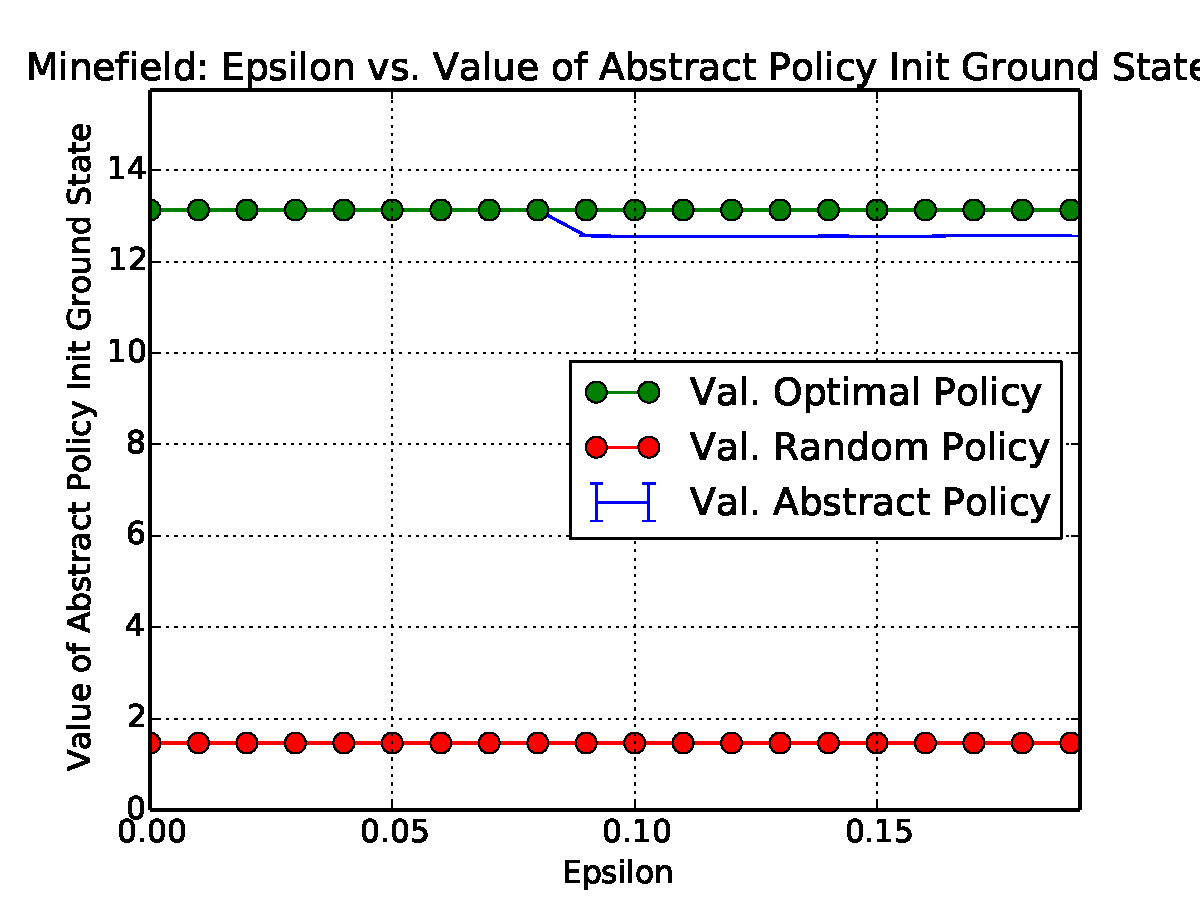
\includegraphics[width=0.46\columnwidth]{figures/minefield_epsilon_vs_value_of_abstract_policy_init_ground_state.pdf}
}

\subfigure[RandomStates]{
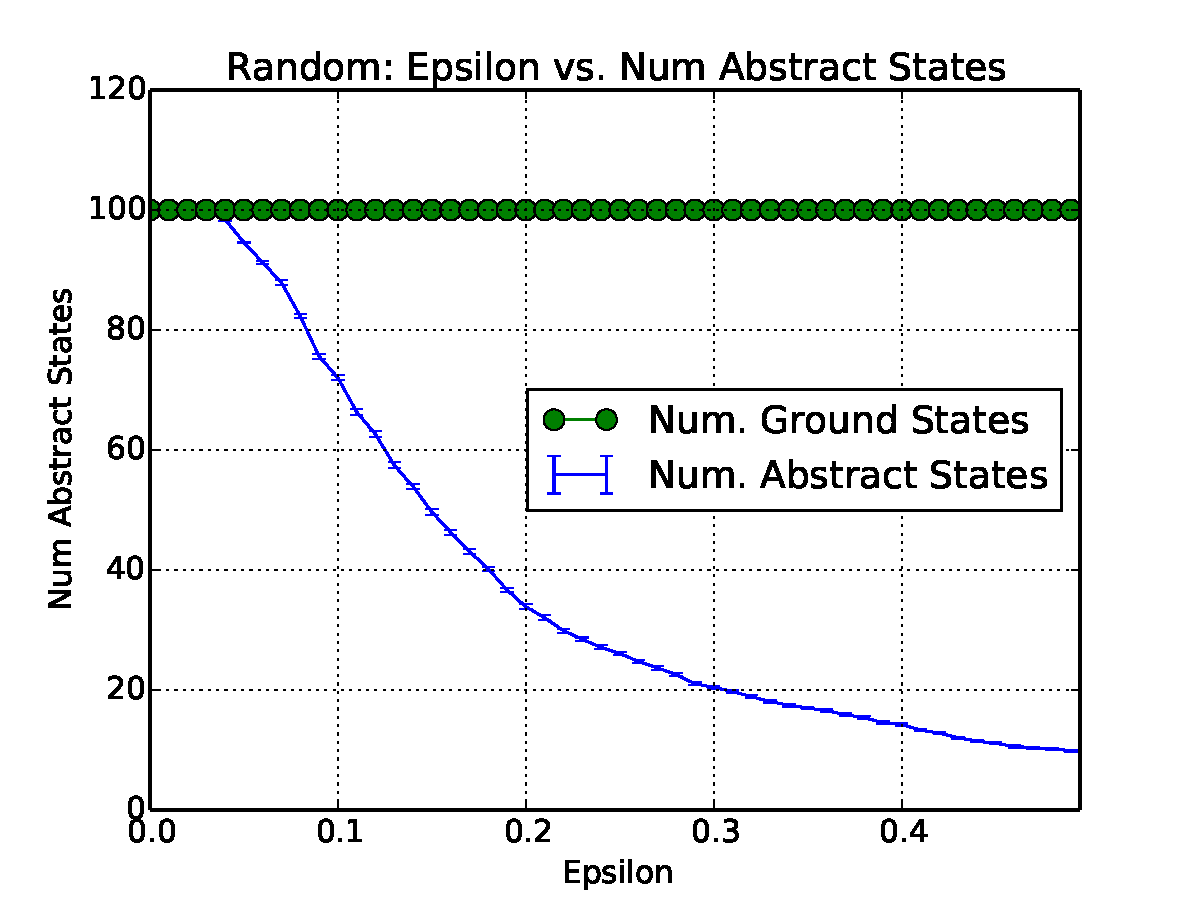
\includegraphics[width=0.46\columnwidth]{figures/random_epsilon_vs_num_abstract_states.pdf}
}
\subfigure[RandomVal]{
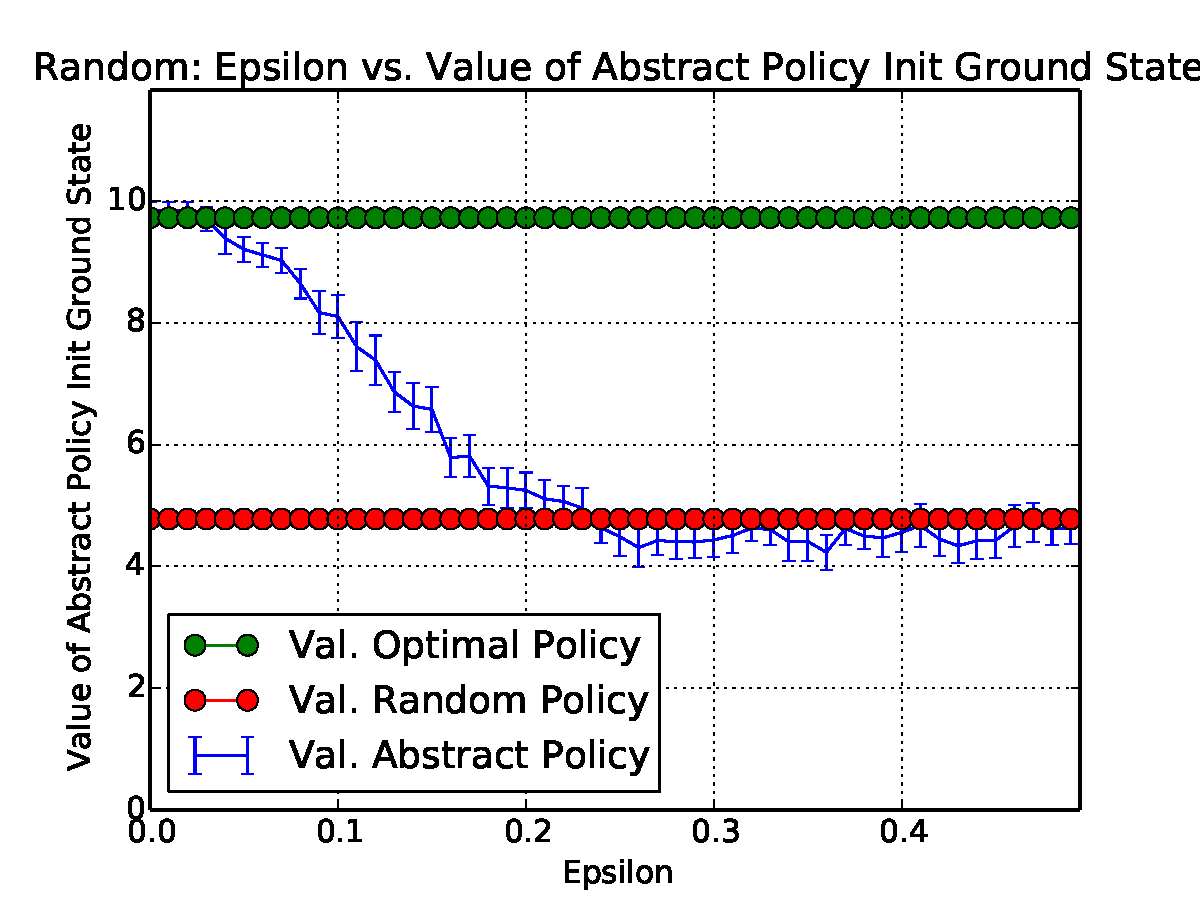
\includegraphics[width=0.46\columnwidth]{figures/random_epsilon_vs_value_of_abstract_policy_init_ground_state.pdf}
}

\label{fig:main results}
\caption{$\epsilon$ vs. Num States and $\epsilon$ vs. Abstract Policy Value}
\end{figure} 
